% Created 2023-11-19 Sun 15:51
% Intended LaTeX compiler: pdflatex
\documentclass[11pt]{article}
\usepackage[utf8]{inputenc}
\usepackage[T1]{fontenc}
\usepackage{graphicx}
\usepackage{longtable}
\usepackage{wrapfig}
\usepackage{rotating}
\usepackage[normalem]{ulem}
\usepackage{amsmath}
\usepackage{amssymb}
\usepackage{capt-of}
\usepackage{hyperref}
\usepackage{xcolor, siunitx}
\author{Hankertrix}
\date{\today}
\title{Physics Electromagnetic Induction Cheat Sheet}
\hypersetup{
 pdfauthor={Hankertrix},
 pdftitle={Physics Electromagnetic Induction Cheat Sheet},
 pdfkeywords={},
 pdfsubject={},
 pdfcreator={Emacs 29.1 (Org mode 9.6.6)}, 
 pdflang={English}}
\begin{document}

\maketitle
\setcounter{tocdepth}{2}
\tableofcontents \clearpage
\section{Definitions}
\label{sec:org83489d0}

\subsection{Magnetic flux}
\label{sec:orga499ff5}
\begin{align*}
\Phi_B &= \int B \cos \phi \, dA \\
&= \int B_{\perp} \, dA \\
&= \int \vec{\boldsymbol{B}} \cdot d \vec{\boldsymbol{A}}
\end{align*}

Where:
\begin{itemize}
\item \(\Phi_B\) is the magnetic flux through a surface.
\item \(B\) is the magnitude of the magnetic field \(\vec{\boldsymbol{B}}\).
\item \(\phi\) is the angle between \(\vec{\boldsymbol{B}}\) and the normal to the surface.
\item \(dA\) is the element of surface area.
\item \(B_{\perp}\) is the component of \(\vec{\boldsymbol{B}}\) perpendicular to the surface.
\item \(d \vec{\boldsymbol{A}}\) is the vector element of the surface area.
\end{itemize}

\subsection{Magnetic flux linkage}
\label{sec:org11830fb}
\begin{align*}
\text{Magnetic flux linkage} &= N \Phi_B \\
&= N \int \vec{B} \cdot d \vec{A} \\
&= NBA \cos \theta
\end{align*}

Where:
\begin{itemize}
\item \(N\) is the number of turns of wire in a coil.
\item \(\Phi_B\) is the magnetic flux.
\item \(\vec{B}\) is the magnetic field.
\item \(d \vec{A}\) is the vector element of the surface.
\item \(B\) is the magnitude of the magnetic field.
\item \(A\) is the area of the surface.
\item \(\theta\) is the angle between the normal to the surface and the magnetic field.
\end{itemize}

\subsection{Faraday's law}
\label{sec:org0514a73}
\begin{enumerate}
\item Faraday's law states that the \textbf{magnitude} of the induced e.m.f is directly proportional to the rate of change of magnetic flux linkage.
\item Or, the law states that the magnitude of the induced e.m.f is directly proportional to the rate of "cutting" of the magnetic flux (motional e.m.f).
\end{enumerate}

\[\mathcal{E} = - N \frac{d \Phi_B}{dt}\]

Where:
\begin{itemize}
\item \(\mathcal{E}\) is the induced e.m.f in a closed loop.
\item \(N\) is the number of turns of the coil.
\item \(\frac{d \Phi_B}{dt}\) is the rate of change of magnetic flux through the loop.
\end{itemize}

Faraday's law refers to induced e.m.f, which makes it applicable to both open and closed circuits.
\\[0pt]

The work done against resistive forces due to induced current is always equal to the internal energy produced in the coil.

\newpage

\subsubsection{Motional e.m.f perspective}
\label{sec:orgec5d16d}

\begin{center}
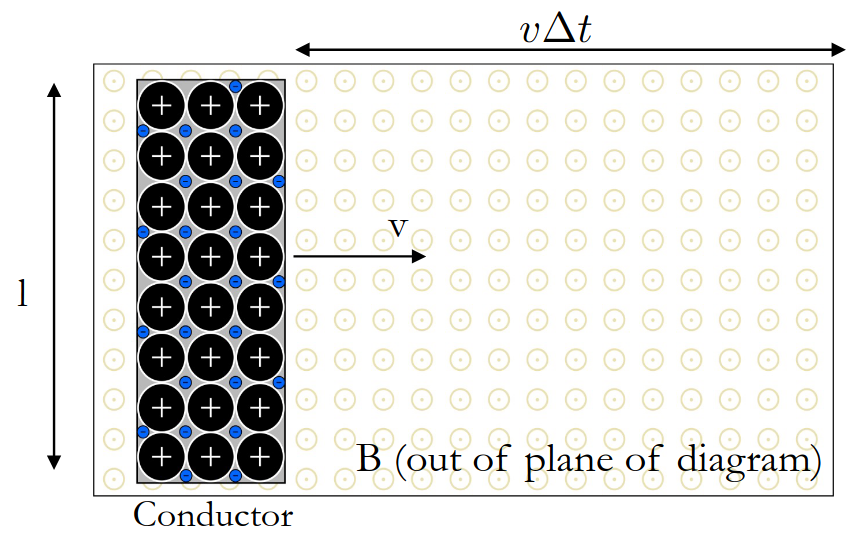
\includegraphics[scale=0.65]{./images/motional-emf.png}
\end{center}

\[\mathcal{E} = Blv\]

Where:
\begin{itemize}
\item \(\mathcal{E}\) is the induced e.m.f.
\item \(B\) is the magnitude of the magnetic field.
\item \(l\) is the length of the conductor.
\item \(v\) is the velocity that the conductor is moving at.
\end{itemize}
Explanation:
\begin{itemize}
\item Electrons in the conductor experiences a force \(\vec{F}_B = q \vec{v} \times \vec{B}\) directed along the length \(l\), perpendicular to \(\vec{v}\) and \(\vec{B}\).
\item As such, electrons accumulate at the upper end of the conductor, leaving a positive charge at the lower end.
\item Thus, an upward electric field \(\vec{E}\) is produced inside the conductor. In equilibrium, the downward magnetic force balances the upward electric force.
\end{itemize}
\[qvB = qE \quad \Rightarrow E = vB\]
\begin{itemize}
\item The potential difference between the ends of the conductor is \(\mathcal{E} = El\). Thus, we get the magnitude of the induced e.m.f, arising from the magnetic force on moving charges:
\end{itemize}
\[\mathcal{E} = Blv\]

\newpage

\subsection{Lenz's law}
\label{sec:org1e9ef01}
Lenz's law states that the direction of any induced e.m.f opposes the change in the magnetic flux that causes it. This law is symbolised by the negative sign in the mathematical form of Faraday's law.
\\[0pt]

Lenz's law is worded to refer to induced current, therefore making it applicable only to closed circuits. If the circuit is open, we can usually think in terms of what would happen if it were closed and hence find the direction of the induced e.m.f.

\subsubsection{Determining the direction of the induced e.m.f}
\label{sec:org01cb5ef}
\begin{center}
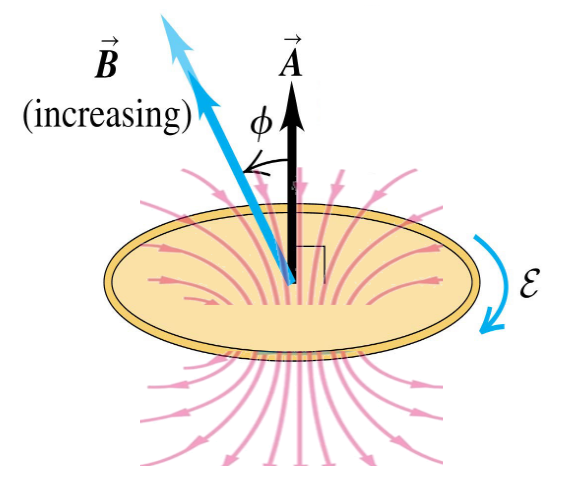
\includegraphics[width=.9\linewidth]{./images/lenz-law.png}
\end{center}

\begin{itemize}
\item Flux is positive (\(\Phi_B > 0\))
\item Flux is becoming more positive \((\frac{d \Phi_B}{dt} > 0)\)
\item Induced e.m.f is in the direction shown above as a closed circuit will allow a corresponding current flow, which would produce an opposing induced magnetic field (\(\textcolor{red}{\text{in red}}\)) within the area of the coil.
\end{itemize}


\subsection{Maxwell's equations}
\label{sec:orgd906638}

\subsubsection{Faraday's Law}
\label{sec:orgf421c80}
\[\mathcal{E} = \oint \vec{E} \cdot d \vec{l} = - \frac{d \Phi_B}{dt}\]

Where:
\begin{itemize}
\item \(\mathcal{E}\) is the induced e.m.f.
\item \(\vec{E}\) is the electric field generated by the changing magnetic field.
\item \(d \vec{l}\) is the vector segment of the path between two points.
\item \(\frac{d \Phi_B}{dt}\) is the change in magnetic flux with respect to time.
\end{itemize}

This equation is true for any closed path, since an electric field is induced at all points in space, and the relation does not need a conductor to close the loop. This also implies that \textbf{electric fields induced by changing magnetic fields are non-electrostatic and non-conservative} as:
\[\oint \vec{E} \cdot d \vec{l} \ne 0\]

\newpage

\subsubsection{Ampere-Maxwell's law}
\label{sec:org34cff03}

\begin{align*}
\oint \vec{B} \cdot d \vec{l} &= \mu_0 \left(I_{enc} + \varepsilon_0 A \frac{dE}{dt} \right) \\
&= \mu_0 \left(I_{enc} + \varepsilon_0 \frac{d \Phi_E}{dt} \right) \\
&= \mu_0 (I_{enc} + I_{disp})
\end{align*}

Where:
\begin{itemize}
\item \(\vec{B}\) is the magnetic field.
\item \(d \vec{l}\) is the vector segment of the path between two points.
\item \(I_{enc}\) is the actual current enclosed by the loop.
\item \(\varepsilon_0\) is the permittivity of vacuum, which is approximately \(8.85 \times 10^{-12} \ \unit{F.m^{-1}}\)
\item \(A\) is the area of the surface the electric field is passing through.
\item \(\frac{dE}{dt}\) is the change of electric field with respect to time.
\item \(\frac{d \Phi_E}{dt}\) is the change of electric flux with respect to time.
\item \(I_{disp}\) is the displacement current.
\end{itemize}

\newpage

\subsubsection{Summary}
\label{sec:org716fa91}

\begin{enumerate}
\item Gauss' law
\label{sec:org47a4a46}
\begin{center}
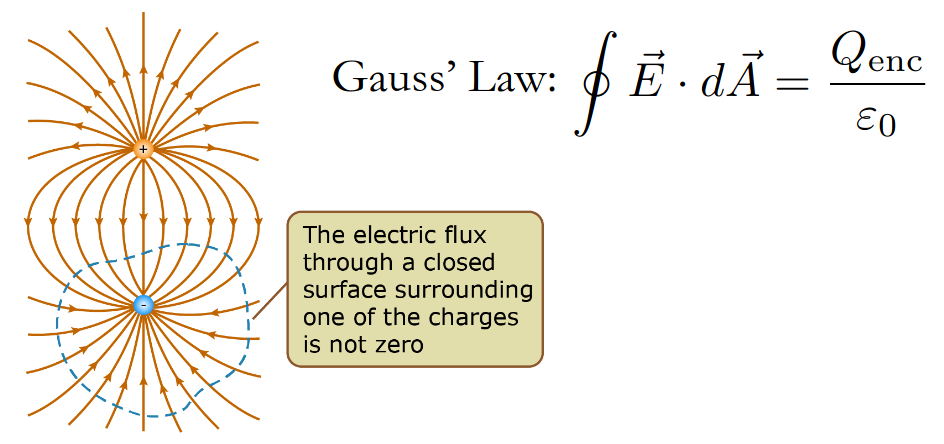
\includegraphics[width=.9\linewidth]{./images/gauss-law.png}
\end{center}

\item Gauss' law for magnetism
\label{sec:org5ffc25e}
\begin{center}
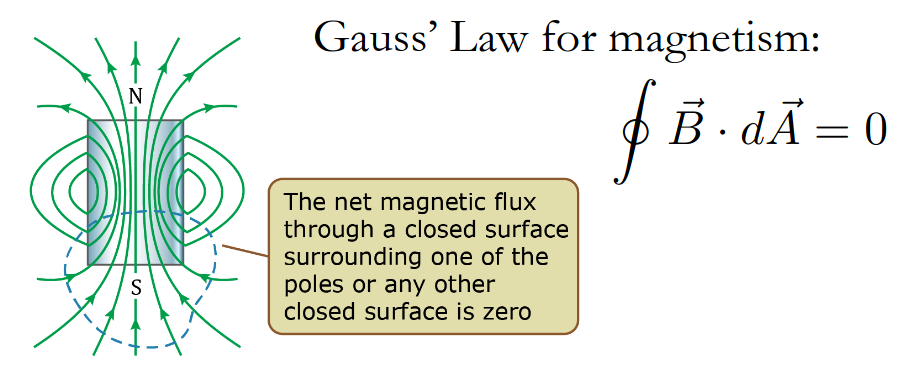
\includegraphics[width=.9\linewidth]{./images/gauss-law-for-magnetism.png}
\end{center}

\item Faraday's law
\label{sec:org600b413}
\begin{center}
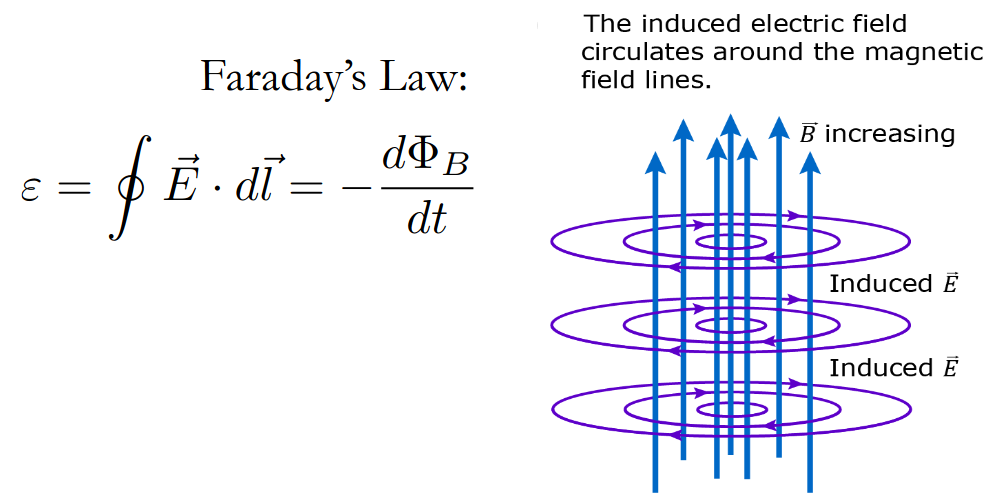
\includegraphics[width=.9\linewidth]{./images/faradays-law.png}
\end{center}

\item Ampere-Maxwell's law
\label{sec:org2f9fbe3}
\begin{center}
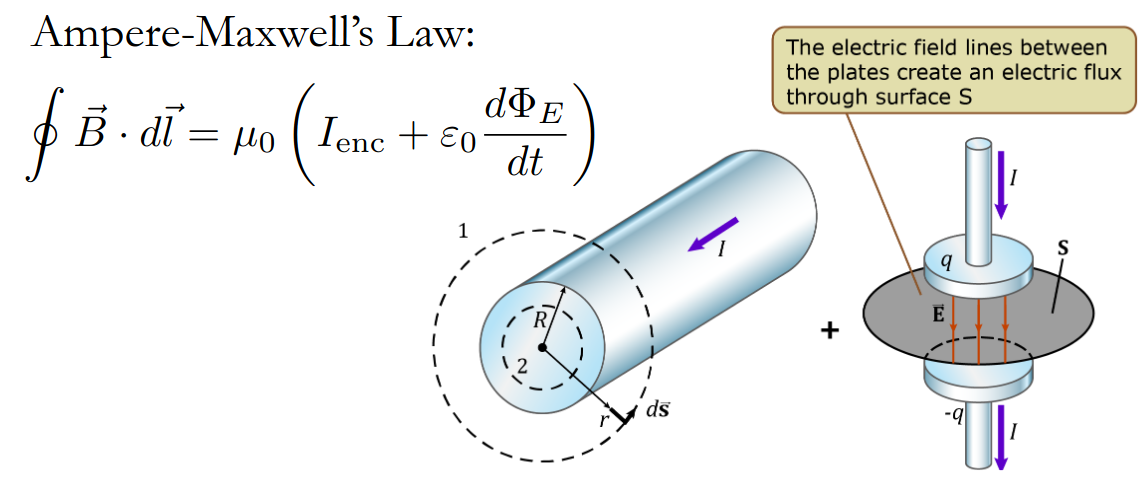
\includegraphics[width=.9\linewidth]{./images/ampere-maxwell-law.png}
\end{center}
\end{enumerate}

\subsection{Mutual inductance}
\label{sec:org48c4267}
\[M = \frac{N_2 \Phi_{B2}}{i_1} = \frac{N_1 \Phi_{B1}}{i_2}\]

Where:
\begin{itemize}
\item \(M\) is the mutual inductance of coils 1 and 2.
\item \(N_2\) is the number of turns in coil 2.
\item \(\Phi_{B2}\) is the magnetic flux through each turn of coil 2.
\item \(i_1\) is the current in coil 1.
\item \(N_1\) is the number of turns in coil 1.
\item \(\Phi_{B1}\) is the magnetic flux through each turn of coil 1.
\item \(i_2\) is the current in coil 2.
\end{itemize}

\subsection{Self inductance}
\label{sec:org4908069}
\[L = \frac{N \Phi_B}{I}\]

Where:
\begin{itemize}
\item \(N\) is the number of turns of the coil.
\item \(\Phi_B\) is the magnetic flux passing through \(N\) turns of the coil.
\item \(I\) is the current in the coil.
\end{itemize}

\subsection{Energy stored in a magnetic field}
\label{sec:org570884c}
\[U_B = \frac{1}{2} L I^2\]

Where:
\begin{itemize}
\item \(U_B\) is the potential energy stored by the inductor in the form of a magnetic field.
\item \(L\) is the self inductance of the inductor.
\item \(I\) is the current in the inductor.
\end{itemize}

\newpage

\section{Applications of electromagnetic induction}
\label{sec:org28c9846}

\subsection{A.C. generators}
\label{sec:orge0fd543}
\begin{center}
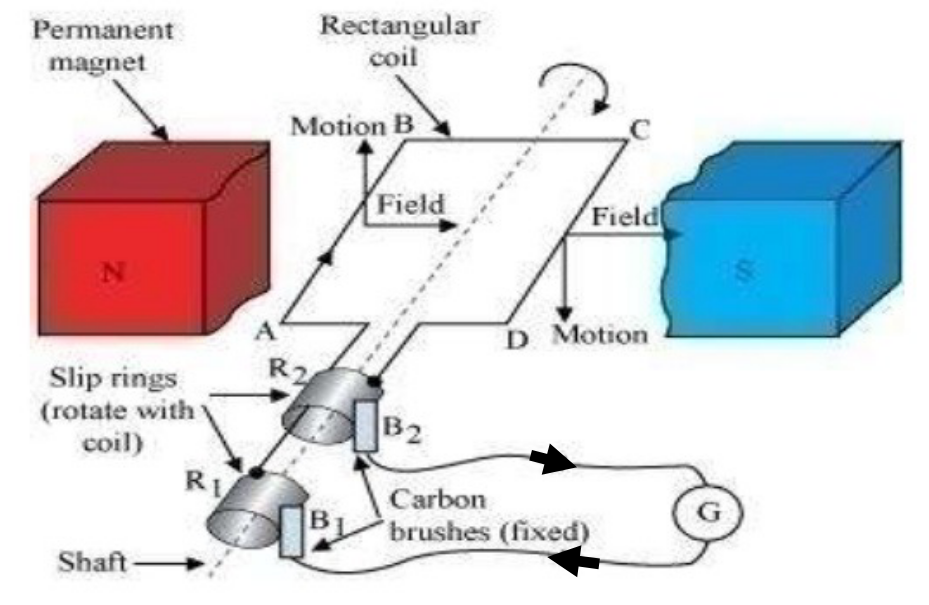
\includegraphics[width=.9\linewidth]{./images/ac-generator.png}
\end{center}

\begin{align*}
\mathcal{E} &= -N \frac{d \Phi_B}{dt} \\
&= -N \frac{d(BA \cos \omega t)}{dt} \\
&= NBA \omega \sin \omega t
\end{align*}

\begin{center}
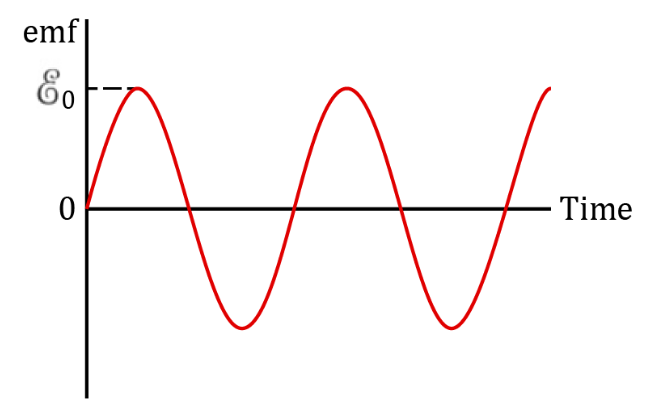
\includegraphics[scale=0.7]{./images/ac-generator-graph.png}
\end{center}

\subsubsection{Half-wave rectifier}
\label{sec:org6569db1}
\begin{center}
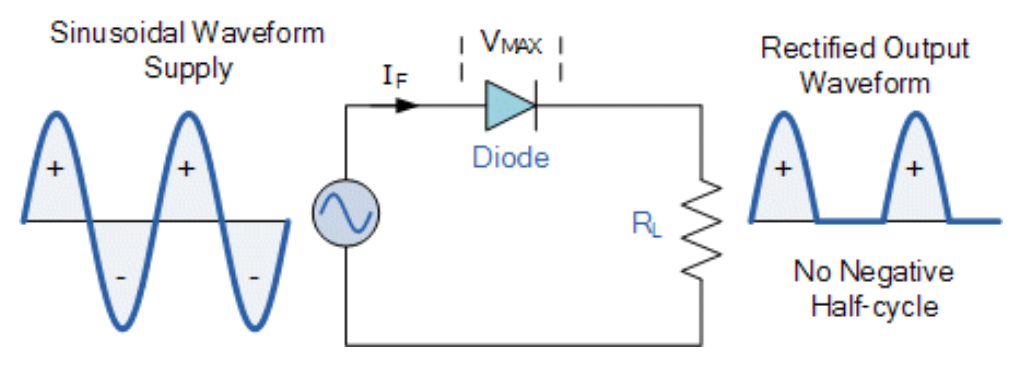
\includegraphics[width=.9\linewidth]{./images/half-wave-rectifier.png}
\end{center}

The current flows through the load resistor from the top to the bottom terminals, for only half of each cycle.

\subsubsection{Full-wave rectifier}
\label{sec:org7cb0257}
\begin{center}
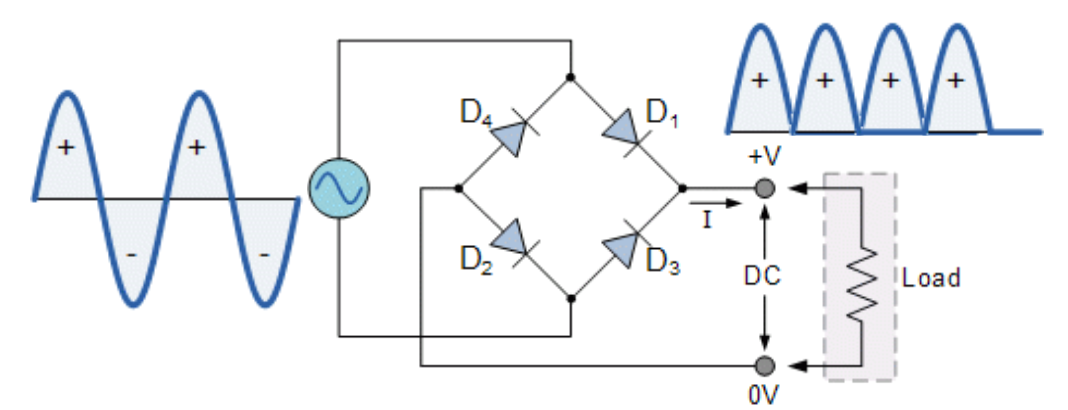
\includegraphics[width=.9\linewidth]{./images/full-wave-rectifier.png}
\end{center}

One can trace the current path through each + or - half cycle to see that the current flows through the load resistor from the top to the bottom terminals for the entire cycle.

\subsubsection{Full-wave rectifier with capacitive smoothing}
\label{sec:org1cd9fdf}
\begin{center}
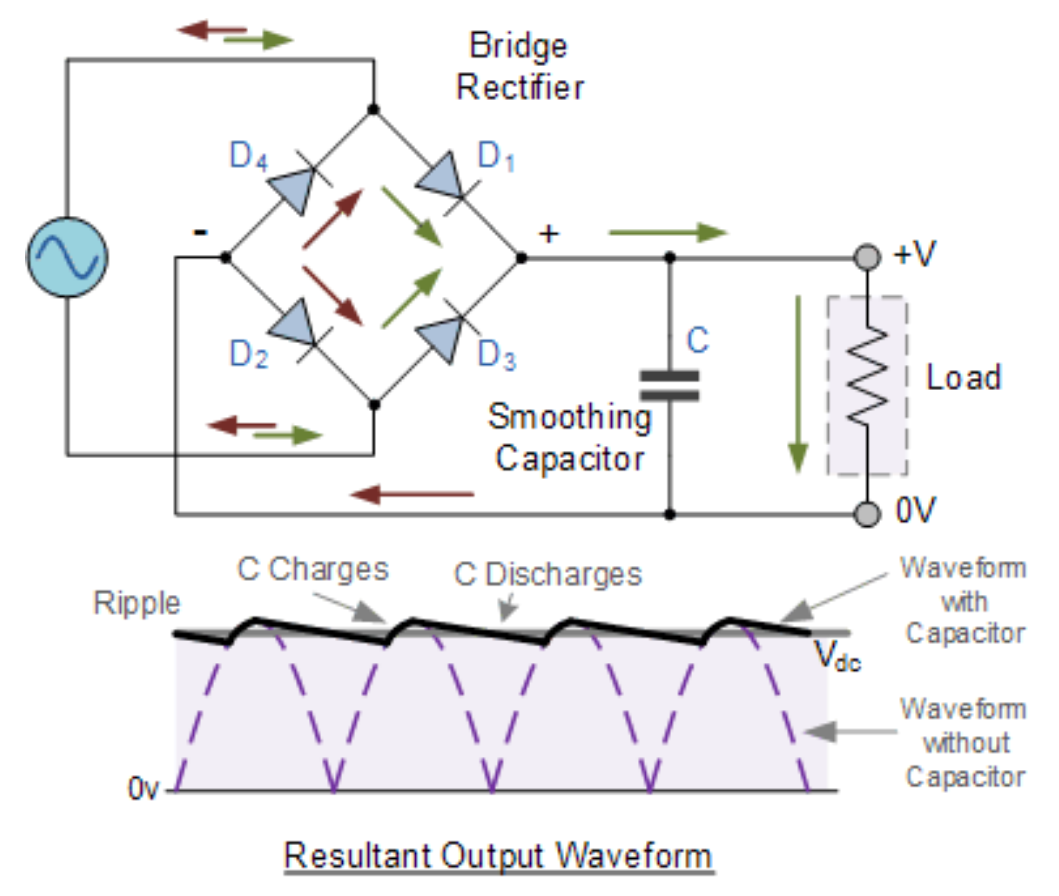
\includegraphics[width=.9\linewidth]{./images/full-wave-rectifier-with-capacitor.png}
\end{center}

The presence of the capacitor smooths the full-wave rectified output.
\\[0pt]

The capacitor charges up as it followed the input sinusoidal voltage. When the input voltage falls below the capacitor's potential difference, it discharges at the time constant \(RC\). A long time constant smoothens the drop in potential difference across the load until the input voltage rises above that of the capacitor's at the next cycle.

\newpage

\subsection{Transformers}
\label{sec:org9b3d5e2}
\begin{center}
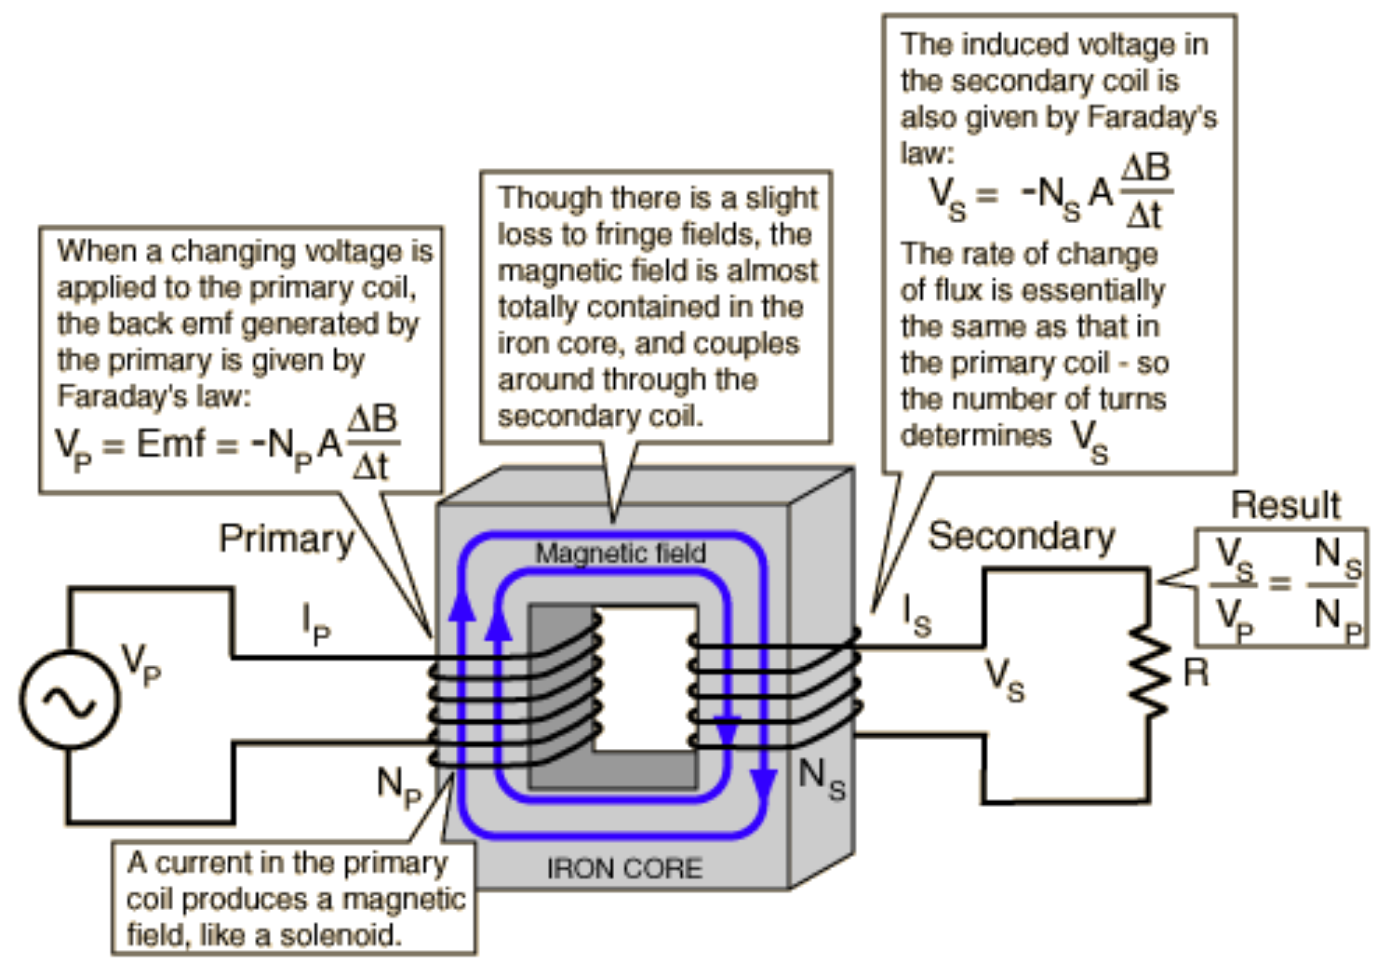
\includegraphics[width=.9\linewidth]{./images/transformers.png}
\end{center}

\[\frac{d \Phi_{B, p}}{dt} = \frac{d \Phi_{B, s}}{dt} \quad \Longrightarrow \quad \frac{V_s}{V_p} = \frac{N_s}{N_p}\]

Where:
\begin{itemize}
\item \(\frac{d \Phi_{B, p}}{dt}\) is the change in magnetic flux in the primary coil.
\item \(\frac{d \Phi_{B, s}}{dt}\) is the change in magnetic flux in the secondary coil.
\item \(V_p\) is the voltage of the primary circuit.
\item \(V_s\) is the voltage of the secondary circuit.
\item \(N_p\) is the number of turns of the primary coil.
\item \(N_s\) is the number of turns of the secondary coil.
\end{itemize}

\newpage

The power supplied to the secondary circuit should ideally be the same as the primary circuit:
\[V_p I_p = V_s I_s\]

Where:
\begin{itemize}
\item \(V_p\) is the voltage of the primary circuit.
\item \(V_s\) is the voltage of the secondary circuit.
\item \(I_p\) is the current of the primary circuit.
\item \(I_s\) is the current of the secondary circuit.
\end{itemize}
\end{document}